% English translation of main.tex for submission to an English-language journal.
% Compile: xelatex main_en.tex (run twice for cross-references)
% Notes:
%  - Chinese-journal-specific front matter (Chinese abstract/keywords, CLC number) removed.
%  - Section numbering follows English convention (Introduction = Section 1), so internal
%    cross-references are handled with \label/\ref rather than hard-coded numbers.
%  - The dialogue example in Table 1 is an English rendering of the original Chinese example.
%  - The reference to "Algorithm 1" in Sec. 4.3.2 is kept from the source manuscript, which
%    contains no corresponding algorithm float.
\documentclass[a4paper,11pt]{article}
\usepackage[T1]{fontenc}
\usepackage{amsmath,amssymb}
\usepackage{graphicx}
\usepackage{booktabs}
\usepackage{caption}
\usepackage[margin=2.5cm]{geometry}
\usepackage[hidelinks]{hyperref}

\title{Latency Optimization of Cascaded Voice Dialogue Systems with a Pipeline-Parallel Streaming Architecture}
\author{}
\date{}

\begin{document}

\maketitle

\noindent\textbf{Abstract}: A pipeline-parallel streaming architecture is proposed to mitigate post-utterance waiting time in cascaded voice dialogue systems for long-form speech. The architecture overlaps speech recognition and language-model prefilling/inference. Voice activity detection enables online segmentation, and an adaptive sliding window with dynamic buffering leverages Whisper timestamp alignment to commit stable transcripts under a prefix--suffix context and a local-consistency constraint. Incremental prefilling with a key--value cache updates only newly arrived text, reducing the time to first token and preventing it from increasing linearly with input length. Experiments on 1,132 progressively-lengthening utterances synthesized from MultiWOZ and CrossWOZ show that mean time to first token remains around 1.1~s in long-utterance groups, achieving 34.6\%--83.9\% reductions over a non-streaming baseline and a 5.67~s average reduction in the longest group, while keeping transcription error rates within an acceptable range. Results indicate that streaming pipeline parallelism and state incrementalization effectively reduce long-utterance interaction latency in modular cascaded systems.

\medskip
\noindent\textbf{Keywords}: streaming architecture; voice dialogue system; pipeline parallelism; incremental prefilling; end-to-end latency

\section{Introduction}

With the development of artificial intelligence, human--computer interaction is evolving from command-style input toward natural spoken dialogue. Although multimodal large models such as GPT-4o and Gemini 1.5 have advanced voice interaction capabilities, deployment cost and engineering maturity still lead most practical systems to adopt a cascaded architecture composed of automatic speech recognition (ASR), a large language model (LLM), and text-to-speech (TTS). For long-form speech, this architecture typically waits for endpoint detection to complete before starting downstream understanding and generation, which introduces post-endpoint waiting latency and degrades the responsiveness and fluency of the interaction.

At the same time, the new generation of voice dialogue systems built on large language models offers stronger understanding, handles complex reasoning, and supports emotionally colored multi-turn natural-language interaction. This higher level of intelligence, however, comes with substantial computational overhead and latency challenges. Published system reports indicate that GPT-4o achieves an end-to-end voice response latency as low as 232~ms, with an average of 320~ms~\cite{ref1}, already approaching human conversational reaction speed. Low latency has therefore become, alongside accuracy, a key competitive metric for the next generation of voice interaction.

Although end-to-end multimodal models perform impressively in papers and experiments, they are expensive to train, complicate data-privacy governance, and require deep customization for vertical scenarios. A cascaded system instead decomposes the pipeline into independent, replaceable modules---voice activity detection (VAD)~\cite{ref2}, ASR, an LLM, and TTS---connected in sequence, and can thus reuse existing high-quality ASR, text LLM, and TTS capabilities. In scenarios that require rapid LLM iteration, controlled deployment cost, and low upgrade risk, the cascaded architecture retains substantial engineering value. In such a serial architecture, the total system latency ($T_{\mathrm{total}}$) depends not only on the processing time of each module but also, to a significant degree, on how data flows between modules. For analysis, the total latency of a serial cascaded system can be expressed as a simple linear sum of the component latencies:
\begin{equation}
T_{\mathrm{total}} = T_{\mathrm{VAD}} + T_{\mathrm{ASR}} + T_{\mathrm{Prefill}} + T_{\mathrm{Decode}} + T_{\mathrm{TTS}} + T_{\mathrm{Net}}
\label{eq:total}
\end{equation}

Here $T_{\mathrm{VAD}}$ denotes the latency of voice activity detection and endpoint decision, $T_{\mathrm{ASR}}$ the speech recognition latency, $T_{\mathrm{Prefill}}$ the latency of the LLM's prefill computation over the input context, $T_{\mathrm{Decode}}$ the decoding latency of the LLM's autoregressive generation, $T_{\mathrm{TTS}}$ the speech synthesis latency, and $T_{\mathrm{Net}}$ the communication overhead of network transmission, request scheduling, and data serialization. Note that the time to first token (TTFT) in this paper measures the system's response time from the end of the user's speech input to the LLM's first generated token; its accounting therefore includes $T_{\mathrm{VAD}}$, $T_{\mathrm{ASR}}$, $T_{\mathrm{Prefill}}$, and the initial decoding latency of the first token, but excludes $T_{\mathrm{TTS}}$ and $T_{\mathrm{Net}}$.

In most conventional cascaded implementations, several seconds may elapse between the end of the user's speech and the system's spoken reply. In long-form scenarios in particular, ASR cannot start until the user finishes the entire utterance, and the LLM's prefill time grows with the length of the input text. How to retain the modularity of the cascaded architecture while using streaming parallelism to shorten the ``dead time'' between modules and approach respond-on-release interaction is therefore of both academic and engineering interest.

\section{Related Work}

\subsection{Streaming Progress in Automatic Speech Recognition}

The processing speed of the ASR system determines how quickly user speech becomes text the LLM can consume. Early streaming ASR architectures were dominated by the RNN-Transducer (RNN-T)~\cite{ref3}. The recurrent nature of RNNs suits streaming audio well, but the step-by-step recurrent dependency limits parallelism over the time dimension during training and makes long-range semantic modeling difficult. With the advent of the Transformer, attention-based models pushed recognition accuracy to new levels~\cite{ref4}. However, the Transformer's global attention requires the entire input before computation can begin, so the vanilla Transformer cannot operate in a streaming fashion.

To address this, Google proposed the Conformer architecture, which combines the local feature extraction of convolutional neural networks (CNNs) with the global modeling of the Transformer and quickly became the industry mainstream~\cite{ref5}. In practice, streaming ASR often uses chunked processing with overlapped stitching: audio is segmented and recognized with a sliding window, and outputs are made consistent across overlap regions, balancing accuracy against latency. Whisper, for example, is an encoder--decoder model aimed primarily at offline transcription~\cite{ref6}; efforts to make such offline models streamable either modify the architecture---converting the non-causal encoder into a causal one so that smaller chunks can be transcribed online at lower latency---or modify the training objective, using sequence-level regularization to encourage earlier token emission and shorten the output lag of streaming recognition.

\subsection{LLM Inference Acceleration}

Once ASR transcription completes, LLM inference speed becomes the second major latency bottleneck, constrained mainly by the autoregressive generation of the Transformer decoder and by GPU memory bandwidth~\cite{ref7}. The key--value cache (KV cache) was introduced precisely to eliminate repeated computation during inference. By caching the Key/Value vectors of historical tokens, the model no longer recomputes intermediate results over the full context when generating a new token, reducing per-step decoding complexity from quadratic to linear in sequence length. The KV cache is now standard in modern inference engines such as vLLM and TGI~\cite{ref8}. For the prefill stage over long inputs, FlashAttention restructures GPU memory access with a tiled computation strategy, raising long-sequence throughput substantially and partially addressing the rapid growth of attention computation with sequence length~\cite{ref9}. For long conversations, StreamingLLM introduces an ``attention sink'' mechanism that anchors early tokens as fixed reference points, mitigating the degradation caused by context-window overflow and allowing the LLM to keep streaming stably within a bounded KV cache.

\subsection{Full-Pipeline Optimization of Voice Dialogue Systems}

Beyond optimizing ASR or the LLM in isolation, coordinated scheduling across the whole pipeline also matters for overall latency. In speech processing tasks such as speech translation, cascaded designs have long been a standard system paradigm: they reuse mature components and allow flexible module replacement, but they also incur intermediate-representation loss, error propagation, and accumulated inter-module latency~\cite{ref10}. Recent end-to-end streaming spoken dialogue models attempt to bypass the traditional ASR--LLM--TTS serial chain, pursuing lower interaction latency through speech-native modeling and streaming generation~\cite{ref11}. Open-source systems such as Mini-Omni, Moshi, and LLaMA-Omni fall into this line of exploration.

\subsection{Contributions of This Work}

\begin{figure}[htbp]
\centering
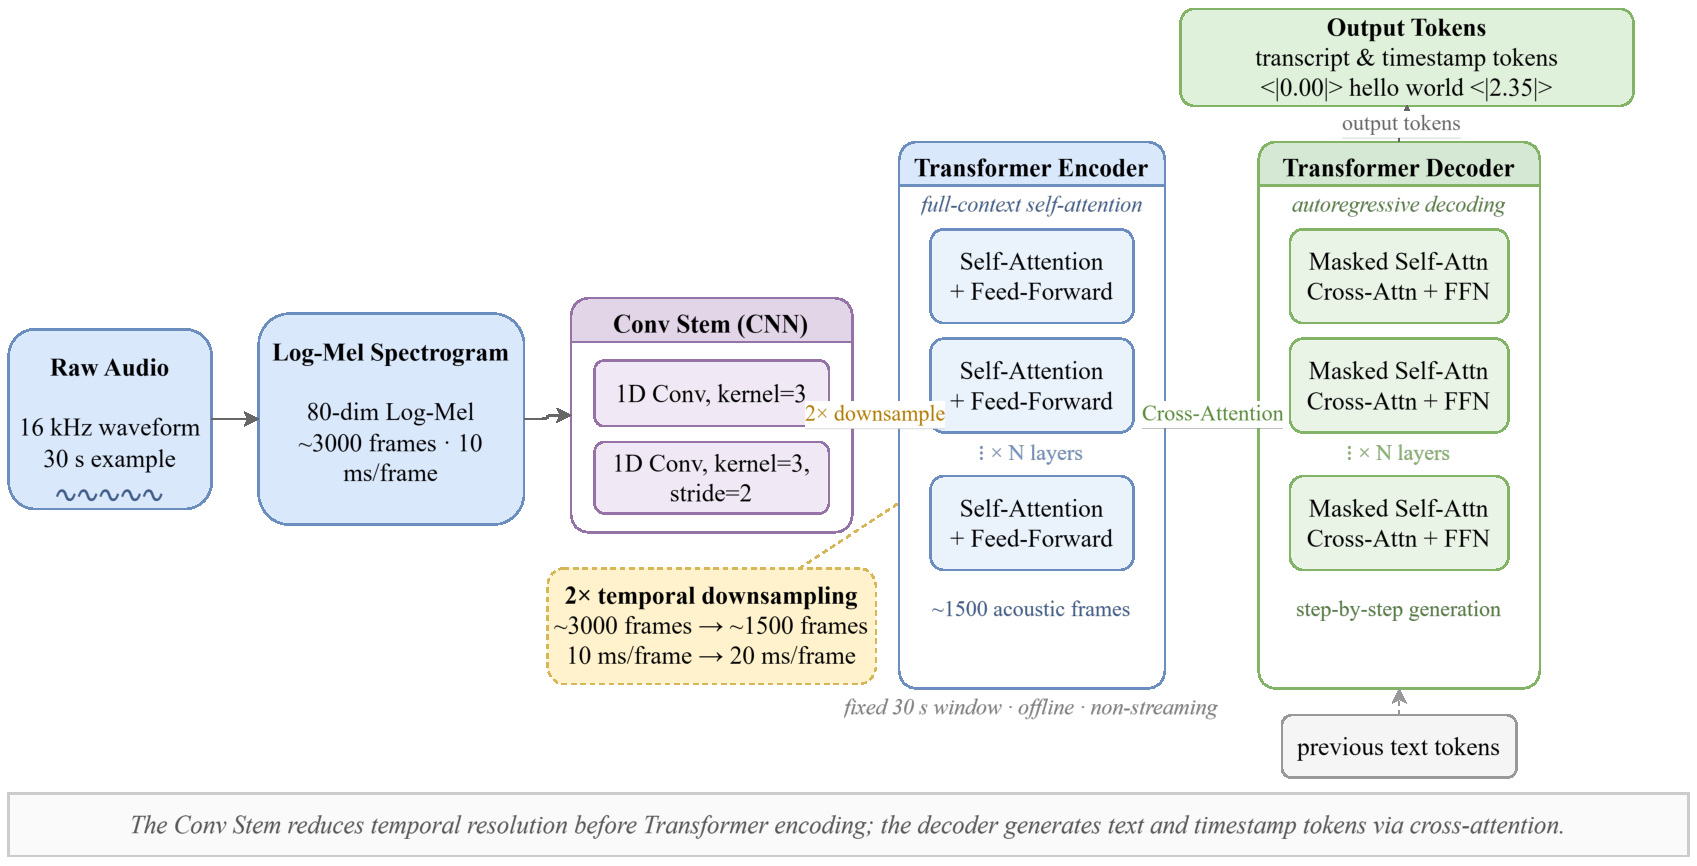
\includegraphics[width=\linewidth]{media/media/image16.pdf}
\caption{Overall architecture of the Whisper model and schematic of feature downsampling}
\label{fig:whisper}
\end{figure}

When a traditional cascaded voice dialogue system processes long speech, per-module latencies accumulate stage by stage while computing resources sit idle. Existing work either optimizes the ASR model alone or extends the LLM into a multimodal architecture that generates speech directly; neither can reuse existing state-of-the-art text models. This paper proposes a fine-grained pipeline-parallel design (hereafter System~B) that is directly compatible with existing non-streaming ASR models and text LLMs. The main contributions are as follows.

A streaming ASR context-management mechanism: we design an adaptive sliding-window algorithm based on Whisper and Silero VAD. To counter the context loss and recognition instability caused by streaming slicing, we propose a dynamic buffering and prefix--suffix context concatenation strategy that preserves long-sentence accuracy while emitting ASR transcript fragments at millisecond-level latency.

Against the first-token latency induced by long speech input, we propose incremental prefilling of streaming transcripts using the LLM's KV cache. The algorithm exploits the Transformer KV-cache mechanism to consume streaming ASR output fragments in real time, performing attention computation and state updates without re-encoding historical context, thereby amortizing the LLM's computation over the user's speaking time.

We build a long-speech benchmark from MultiWOZ (English) and CrossWOZ (Chinese) and use it for full-pipeline end-to-end latency evaluation (construction details are given in Section~\ref{sec:data}). Experimental results show that for utterances longer than 15 seconds, the proposed System~B significantly reduces latency relative to the traditional non-streaming baseline (hereafter System~A) without degrading the system's semantic understanding.

\section{Principles and Methods}

\subsection{Automatic Speech Recognition}

\subsubsection{Whisper Architecture and Its Offline Nature}

We adopt OpenAI's Whisper as the speech-to-text module. Whisper is an end-to-end Transformer encoder--decoder model that outputs text tokens directly from speech features. Pretrained on large-scale weakly supervised speech--text data, it is robust across languages, accents, and noise conditions~\cite{ref12}.

As shown in Figure~\ref{fig:whisper}, Whisper converts 16~kHz audio into 128-dimensional log-Mel spectrogram features (consistent with the Whisper-Turbo, i.e., large-v3-turbo, model used in our experiments; earlier Whisper models use 80 dimensions), downsamples them through a convolutional front end, and feeds them to a Transformer encoder; the decoder reads the encoder representations through cross-attention and autoregressively emits text tokens. Its vocabulary includes timestamp tokens that provide segment- or word-level alignment, which underpins our strategy of committing only stable, alignable partial outputs in streaming scenarios. Note, however, that Whisper's default interface still favors offline processing of fixed-length segments, which is exactly what makes streaming adaptation challenging.

\subsubsection{Streaming Challenges and Our Approach}

Whisper's encoder self-attention can exploit both past and future frames, which helps accuracy offline but creates two difficulties in real-time dialogue: first, when short chunks are recognized independently, words near chunk boundaries are prone to omission, repetition, or rewriting; second, the trailing hypothesis keeps changing as subsequent audio arrives, so a downstream LLM cannot consume it stably.

We address both problems with a combined strategy of segmented input, overlapped context, and stable commitment: the front end uses VAD to detect and split the continuous PCM stream into speech segments; the ASR side retains context before and after the target segment to mitigate boundary information loss; and the output side uses Whisper's word-level timestamps to commit only text lying in a stable region, providing the LLM's incremental prefilling with a consumable text stream.

\subsection{LLM Inference}

\subsubsection{Transformer Attention}

Large language models typically adopt a decoder-only Transformer architecture. In a voice dialogue system, LLM inference latency---first-token latency in particular---is the key bottleneck determining whether the user perceives lag. From the standpoint of the inference pipeline, TTFT consists mainly of the prefill computation over the input prompt plus the first decoding step, and the cost of both is closely tied to input sequence length. The core of the Transformer is scaled dot-product attention:
\begin{equation}
\mathrm{Attention}(Q,K,V)=\mathrm{softmax}\!\left(\frac{QK^{\top}}{\sqrt{d_k}}\right)V
\label{eq:attention}
\end{equation}

Here $Q$ (Query), $K$ (Key), and $V$ (Value) are obtained from the input vectors through linear projection matrices $W_Q$, $W_K$, and $W_V$, respectively. The Key dimension $d_k$ rescales the dot products so that $QK^{\top}$ does not suffer variance inflation as dimensionality grows, which would saturate the softmax and shrink gradients. This mechanism lets the model aggregate information from any position of the sequence within a single time step, capturing long-range dependencies.

\subsubsection{KV Cache: Mathematical Principle and Complexity}

Text generation in an LLM is inherently autoregressive: to generate the $N$-th token, the model uses the context of the preceding $N-1$ tokens. In the self-attention module, a single forward pass over a sequence of length $N$ costs $O(N^{2})$. The total computation to generate a sequence of length $N$ is therefore
\begin{equation}
T_{\mathrm{total}}^{\mathrm{naive}}=\sum_{t=1}^{N}O(t^{2})=O\!\left(\frac{N(N+1)(2N+1)}{6}\right)\approx O(N^{3})
\label{eq:naive}
\end{equation}

Modern inference frameworks do not literally repeat full forward passes, but the expression makes the source of redundant computation in autoregressive generation clear: every step recomputes the Key/Value of historical tokens and their attention interactions. The KV cache simply stores these historical values for reuse in later decoding. Because model parameters are fixed at inference time, the $K_i$ and $V_i$ of a historical token $x_i\ (i<t)$ never change once computed and can be stored in GPU memory. At generation step $t$, the system only computes $k_t$ and $v_t$ for the current token $x_t$ and appends them to the cache:
\begin{equation}
K_{\mathrm{cache}}^{(t)}=\mathrm{Concat}\left(K_{\mathrm{cache}}^{(t-1)},\,k_t\right)
\label{eq:kcache}
\end{equation}
\begin{equation}
V_{\mathrm{cache}}^{(t)}=\mathrm{Concat}\left(V_{\mathrm{cache}}^{(t-1)},\,v_t\right)
\label{eq:vcache}
\end{equation}

Attention then involves only the interaction of the current query $q_t$ with the cached history $K_{\mathrm{cache}}$ and $V_{\mathrm{cache}}$: compute $q_t K_{\mathrm{cache}}^{\top}$ and take the weighted sum over $V_{\mathrm{cache}}$. The KV cache thus lowers the per-step decoding complexity from $O(t^{2})$ to $O(t)$---still linear in context length---so the cumulative cost of generating $N$ tokens is about $\sum_{t=1}^{N}O(t)=O(N^{2})$, at the price of cache memory that grows linearly with sequence length.

We emphasize that the KV cache plays two roles in this paper. First, during LLM decoding it reuses the Key/Value already computed for historical tokens, avoiding repeated forward passes over the full context for every new token and reducing the redundant cost of autoregressive decoding. Second, in our streaming architecture, ASR text does not arrive all at once after the speech ends; it is produced progressively as the user speaks. The system can therefore split the prompt prefill that would otherwise happen entirely after the end-of-speech endpoint into multiple incremental prefills: whenever a new stable transcript fragment arrives, only the new text is run through a forward pass and its Key/Value appended to the cache. Incremental prefilling does not eliminate the attention computation the Transformer needs for context modeling, nor does it change the theoretical complexity order of processing the full input. Its benefit lies in the re-timing of computation: most of the prefill for a long prompt is moved forward into the user's speaking time, overlapping with ASR and audio input, which shortens the wait between endpoint detection and first-token generation---that is, the user-perceived TTFT. Figure~\ref{fig:kvcache} contrasts the computation paths of conventional one-shot prefilling and our incremental prefilling with KV-cache reuse.

\begin{figure}[htbp]
\centering
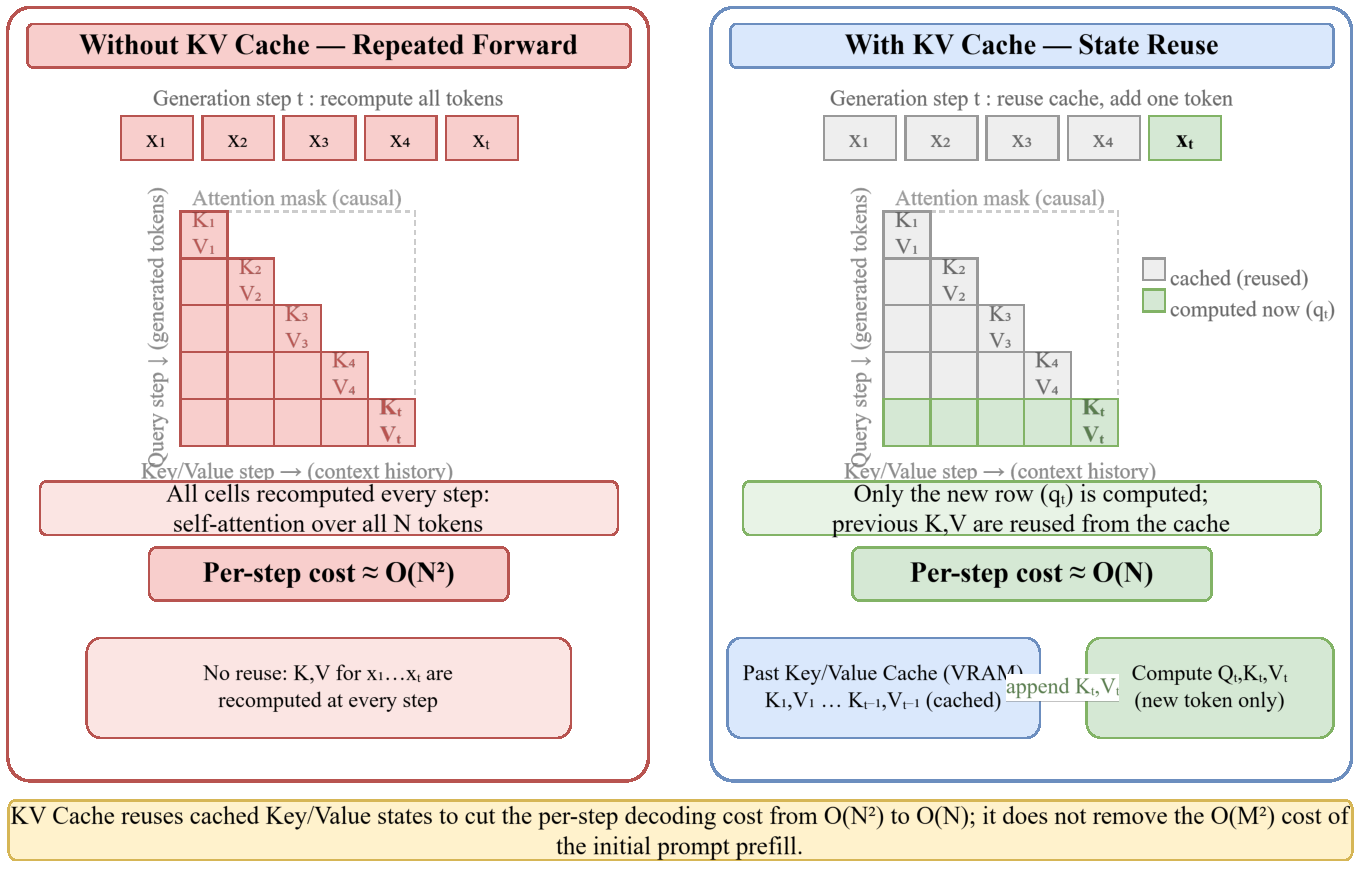
\includegraphics[width=0.85\linewidth]{media/media/image35.pdf}

(a) System A: naive inference (no cache)\qquad (b) System B: incremental inference (KV cache)
\caption{Schematic of the KV Cache-based inference mechanism}
\label{fig:kvcache}
\end{figure}

\subsection{Evaluation Metrics}

\subsubsection{Time to First Token}

TTFT is the core metric of interaction responsiveness and directly reflects the user's subjective waiting experience. We define TTFT as the time difference between the end-of-speech endpoint and the LLM's first output token, treating it as the aggregate latency of the post-endpoint critical path. In System~B, part of the prefill computation is moved forward by the incremental prefilling strategy and runs in parallel with ASR while the user is still speaking, so the post-endpoint wait is expected to drop significantly relative to System~A.

\subsubsection{Word Error Rate}

Although the primary goal of this work is lower latency, it must not come at the cost of recognition accuracy. Word error rate (WER), the standard metric for ASR accuracy, is computed from the Levenshtein edit distance:
\begin{equation}
\mathrm{WER}=\frac{S+D+I}{N_{\mathrm{ref}}}
\label{eq:wer}
\end{equation}

where $S$, $D$, and $I$ are the numbers of substitution, deletion, and insertion errors, and $N_{\mathrm{ref}}$ is the total word count of the reference text. WER is usually reported as a percentage (multiplying by 100\%). For the Chinese dataset we primarily examine the character error rate (CER), whose computation is identical in logic to WER.

\section{System Design}

\subsection{Overall Architecture}

\subsubsection{Objective and Logical Topology}

The core design objective is to shift from the traditional ``receive everything, then process everything'' paradigm to an ``incremental receive, streaming process'' paradigm, minimizing first-token latency at the theoretical boundary. The logical topology is shown in Figure~\ref{fig:topology}, which depicts the streaming parallel data flow built on multi-threaded producer--consumer queues. Audio enters the segmentation module continuously as fixed-length PCM chunks; Silero VAD performs activity detection on an accumulation buffer and emits speech segments~\cite{ref13}. The ASR module concatenates several speech segments, invokes Whisper for transcription, and emits stable text fragments according to the prefix/suffix context policy. Text fragments are passed through a thread-safe queue to the LLM module, which keeps updating the KV cache and starts generation when the termination marker arrives, thereby moving as much LLM prefill computation as possible forward to overlap with audio input.

The overall architecture is a segment--transcribe--prefill--generate pipeline: as soon as an upstream module produces a new audio or text segment, the downstream module can start computing without waiting for the full input. The system comprises three subsystems: a Streaming Audio Segmenter for voice activity detection and segmentation, a Context-Aware ASR Engine for context concatenation and output stability, and an Incremental LLM Inference Service for incremental prefilling and final generation. The KV cache in the LLM part is a general optimization for Transformer decoder inference; we directly reuse the \texttt{past\_key\_values} mechanism built into the inference framework for state reuse.

\subsubsection{Key Engineering Details}

To keep the streaming pipeline real-time and controllable in a single-machine prototype, the implementation splits the chain into a multi-threaded pipeline decoupled by thread-safe queues, with state objects carrying cross-segment context.

For communication, modules do not call each other synchronously; they communicate asynchronously through a producer--consumer model. In the implementation, the audio-chunk queue, audio-segment queue, and text-segment queue are all instances of \texttt{queue.Queue}; consumers loop on \texttt{get} with a timeout, and a designated end-event marks the end of production, avoiding single-point blocking that could deadlock the pipeline. In the ASR stage, the system must simultaneously accept segmented audio from upstream and stream transcribed text downstream, so it is split into two sub-threads, a collector and a transcriber: the former continuously receives upstream speech segments and writes them to a waiting queue; the latter, when the trigger condition is met, concatenates them in batch, calls Whisper for transcription, and pushes the stable portion of the transcript to the downstream LLM, decoupling audio collection from model inference.

\begin{figure}[htbp]
\centering
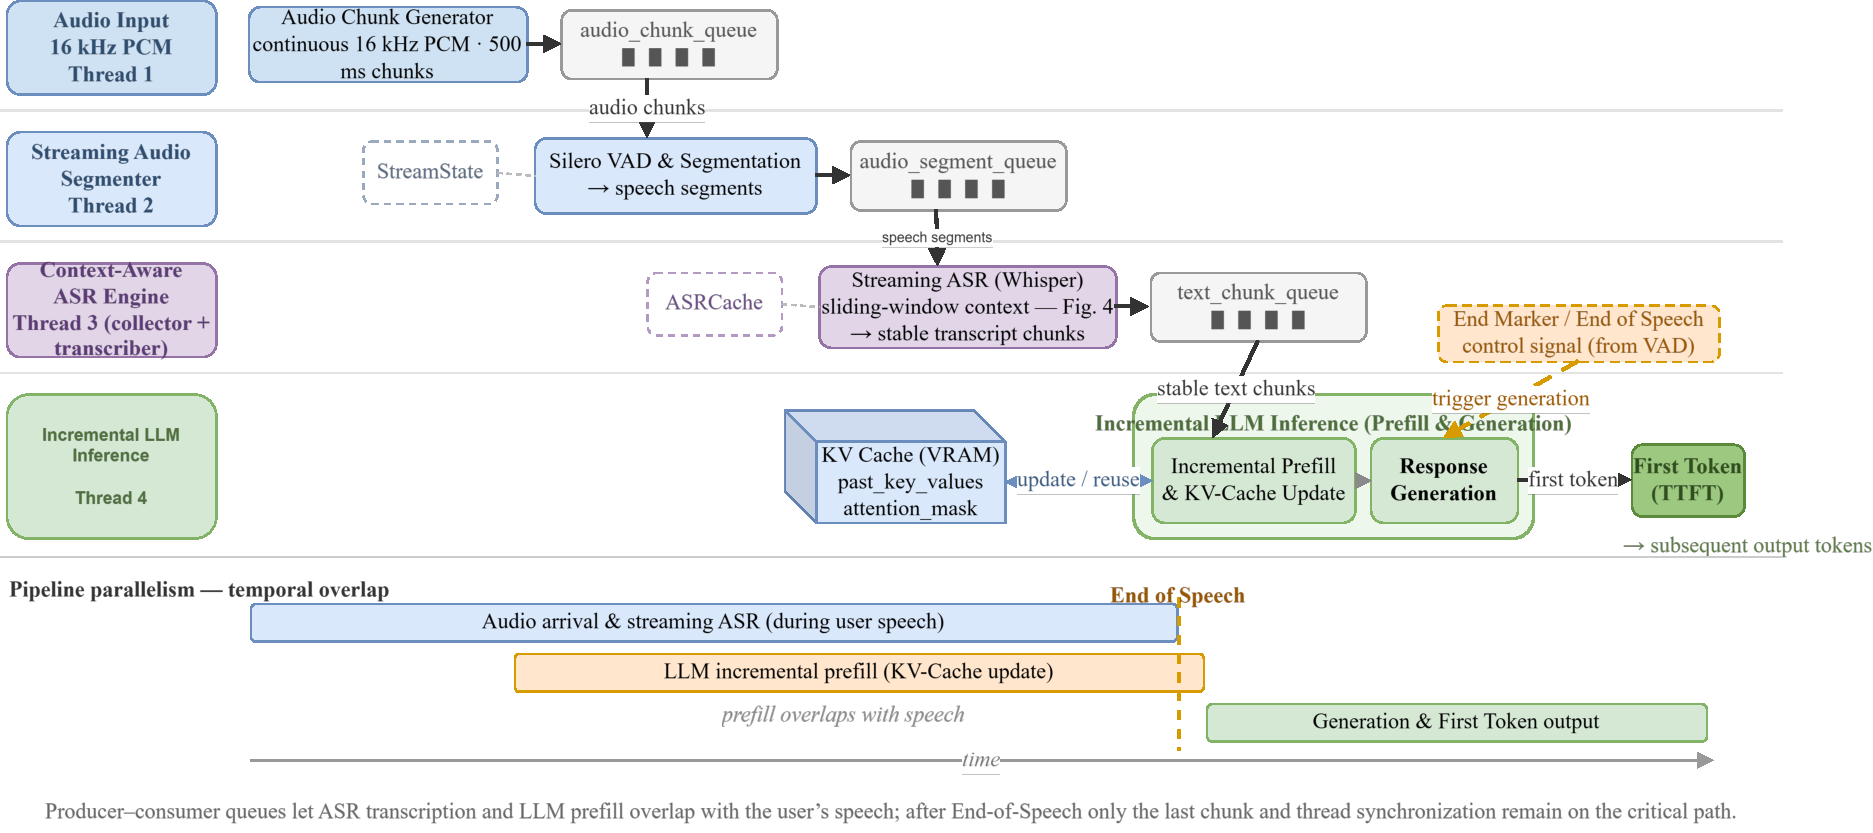
\includegraphics[width=\linewidth]{media/media/image40.pdf}
\caption{Logical topology of the streaming parallel architecture}
\label{fig:topology}
\end{figure}

State management uses a hybrid stateful/stateless design. The segmentation module maintains the accumulated audio buffer, segment start/end times, and segment indices in a \texttt{StreamState} object. The ASR side manages the waiting queue and the current transcription-window queue in an \texttt{ASRCache}, using \texttt{total\_duration} and processing flags to avoid concurrent races. The LLM side persists \texttt{past\_key\_values} and \texttt{attention\_mask} in a \texttt{KVCache}, together with the last-step \texttt{logits} produced during prefilling, so that generation can start immediately when the termination marker arrives. These state objects jointly guarantee cross-segment context consistency and ground the algorithm descriptions in Sections~\ref{sec:asr-context} and~\ref{sec:kv-prefill}.

\subsection{Streaming ASR Context Management}
\label{sec:asr-context}

\subsubsection{Strategy}

The central challenge of streaming ASR is the optimal balance between recognition accuracy and latency: slices that are too short deprive the model of necessary acoustic context, and the resulting lack of inductive bias sharply increases the word error rate; waiting for slices that are too long introduces significant buffering and processing delay, eroding the advantage of streaming. This section presents an adaptive context-management strategy based on a dynamic sliding window.

\subsubsection{Dynamic VAD Segmentation}

The system uses the Silero VAD model to segment the continuous PCM stream online. Define the input audio stream as a time series $\{x_1,x_2,\dots,x_t\}$. The segmenter maintains an accumulation buffer $A_{\mathrm{accum}}$ and, on receiving each new audio chunk $c_t$, performs $A_{\mathrm{accum}}\leftarrow A_{\mathrm{accum}}\oplus c_t$, where $\oplus$ denotes concatenation. Once the accumulated audio exceeds the minimum detection window, Silero VAD is invoked; if sufficiently long silence is detected and the speech segment exceeds the minimum speech threshold, the segment is considered closed and emitted to the downstream ASR. The prototype uses a 500~ms chunk length, a 2~s minimum speech length, and a 300~ms minimum silence duration. These values trade off responsiveness against segmentation stability: the 500~ms chunk gives fine online detection granularity while avoiding the frequent VAD calls and thread-scheduling overhead of shorter chunks; the 2~s minimum speech length ensures each fragment submitted to Whisper has enough context, reducing the instability of very short fragments; and the 300~ms silence threshold distinguishes intra-sentence pauses from true end of speech, preventing premature truncation. In terms of sensitivity, smaller chunks or silence thresholds shorten endpoint-detection waiting but may increase spurious segmentation and boundary jitter; larger chunks, minimum speech lengths, or silence thresholds improve stability but increase post-endpoint waiting. We therefore fix these VAD parameters in all comparison experiments to keep configurations comparable.

\subsubsection{Sliding-Window Context Awareness}

\begin{figure}[htbp]
\centering
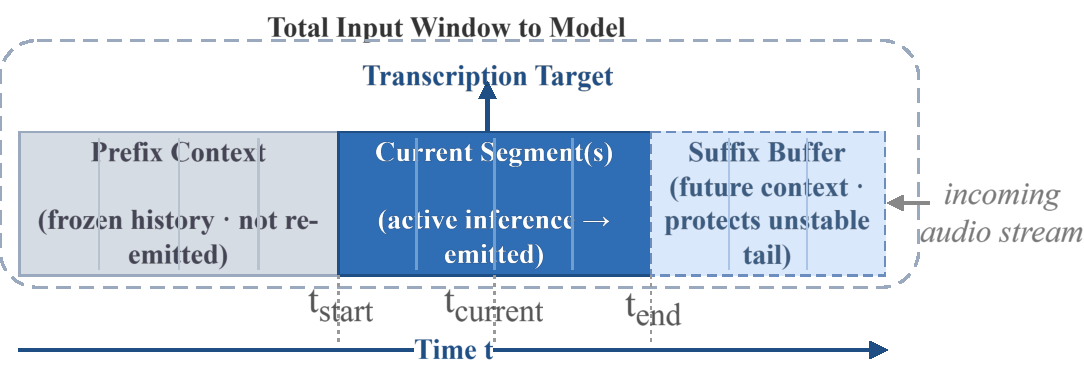
\includegraphics[width=0.55\linewidth]{media/media/image50.pdf}
\caption{Schematic of the context-aware ASR sliding-window mechanism}
\label{fig:window}
\end{figure}

To counter boundary effects in streaming recognition, the ASR engine uses a sliding window that includes prefix context. Figure~\ref{fig:window} details the model input at time step $t$. The window is divided into three logical regions: the prefix context is frozen history that supplies necessary acoustic background; the current segment is the target region for inference; and the suffix buffer holds future audio to prevent truncation effects. This overlapped slicing preserves the coherence of streaming recognition output.

First, the window is updated. Let $Q_t$ be the audio-segment queue at time $t$. Newly arrived segments first enter a waiting queue and are then merged in batch into the main queue by the transcription thread, yielding $Q_t$. Transcription is triggered when the accumulated queue duration reaches the threshold $\tau_{\mathrm{asr}}$ and the queue length satisfies Eq.~(\ref{eq:trigger}):
\begin{equation}
\left|Q_{\mathrm{temp}}\right|\geq N_{\mathrm{prefix}}+1+N_{\mathrm{suffix}}
\label{eq:trigger}
\end{equation}

where $\left|Q_{\mathrm{temp}}\right|$ is the current temporary queue length and $N_{\mathrm{prefix}}$ and $N_{\mathrm{suffix}}$ are the configured numbers of preceding and following segments. When the condition is met, or when the final speech segment arrives, the ASR model concatenates all segments in the temporary queue and performs one transcription pass to produce the raw transcript. In practice a minimum-recognition threshold is also applied to avoid the frequent calls and unstable output caused by overly short windows.

Second, deterministic text extraction is performed. ASR models such as Whisper exhibit ``flicker'' at the tail of streaming input: as new audio arrives, previously emitted trailing words may change. The system therefore adds a suffix-protection region on the output side and emits only text within the stable region between the prefix and suffix segments. To keep output aligned with audio segments, our implementation uses Whisper's word-level timestamps to map words in the raw transcript back to each segment's time span by their end times, producing segment-level candidate text; only the text of segments inside the stable region is concatenated as this round's output. The implementation handles stream boundaries specially: in the first round, no prefix has been emitted, so the stable region may start from zero; in the final round, all remaining segments are emitted so no text is left behind. Finally, the buffer state migrates. After emitting the stable-region text, the window slides to bound accumulated length and preserve acoustic continuity: rather than clearing the queue, the system keeps the $N_{\mathrm{prefix}}$ segments preceding the last emitted segment as the next round's prefix context and retains the not-yet-emitted suffix-protection segments. Note that the cost of stable output is not merely one extra slice of fixed delay; at least $N_{\mathrm{suffix}}$ subsequent segments must arrive and the trigger threshold $\tau_{\mathrm{asr}}$ must be met. In exchange, boundary text becomes stable and accurate, allowing the downstream LLM to prefill incrementally with confidence---a controlled end-to-end latency reduction at the system level without sacrificing input accuracy.

\subsection{Incremental KV-Cache Prefilling for the LLM}
\label{sec:kv-prefill}

\subsubsection{Strategy}

In System~A, the LLM obtains the complete prompt only after ASR finishes transcribing the whole utterance, and performs prefill plus first-token generation entirely after the end-of-speech endpoint. TTFT therefore rises markedly as transcript length grows. Applying that serial paradigm unchanged to a setting where computation could proceed during audio input wastes the time window before the endpoint and squanders the available parallelism.

To reduce post-endpoint computation and support pipeline parallelism, System~B introduces incremental prefilling in the LLM: before the endpoint, the streaming text produced so far is preprocessed, and the \texttt{past\_key\_values} generated by the Transformer decoder's prefill are kept in memory or GPU memory as the KV-cache history. When a new text fragment arrives, the saved \texttt{past\_key\_values} are reused, a forward pass is run only over the new tokens, and the updated \texttt{past\_key\_values} replace the old ones; the process repeats for each subsequent fragment. Most of the LLM's incremental prefilling thus completes while the user is still speaking. When the termination marker arrives, the system only needs to process the final fragment and can immediately start computing the reply tokens, shortening the wait from end of speech to first token.

\subsubsection{Core Algorithm}

The core logic of incremental inference: on the first call, the system performs a one-shot prefill without any cache, establishing the initial KV cache; thereafter, each new ASR text fragment from upstream triggers a call to \texttt{cache\_prompt()}, which updates incrementally on top of the existing \texttt{past\_key\_values}. When the termination marker is received, the system appends the generation prompt (e.g., ``assistant:'', telling the model that the next output token begins the assistant's reply) to the end of the prompt and reuses the last-step logits from prefilling to start decoding directly. To avoid positional-encoding misalignment of incremental tokens, the implementation constructs \texttt{position\_ids} explicitly and encodes new fragments without adding another generation prompt, keeping cache concatenation controlled. Algorithm~1 gives the incremental update procedure corresponding to this implementation. Figure~\ref{fig:kvupdate} visualizes the state changes in GPU memory: the blue region on the left is the cached key--value pairs of the historical context, and the green region on the right is the key--value pairs produced by the new fragment. On each fragment's arrival, incremental prefilling reuses the historical \texttt{past\_key\_values} and runs the forward pass only over new tokens before updating the cache, avoiding repeated prefills over the full prompt in the incremental setting.

\begin{figure}[htbp]
\centering
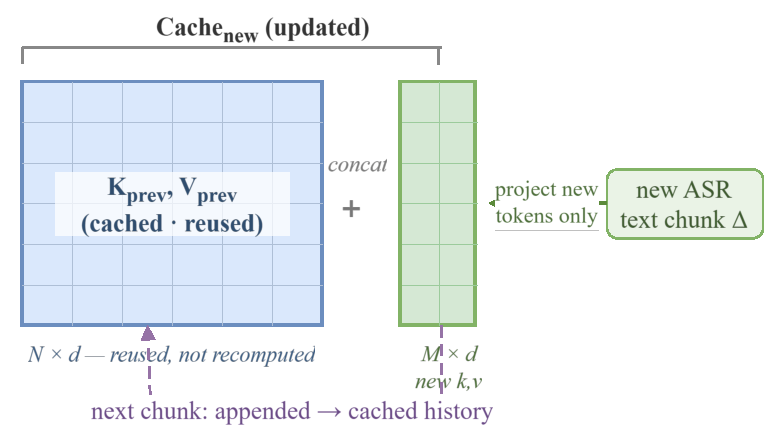
\includegraphics[width=0.55\linewidth]{media/media/image64.pdf}
\caption{Schematic of the LLM KV Cache incremental update mechanism}
\label{fig:kvupdate}
\end{figure}

\subsubsection{Complexity Analysis}

To locate the source of the redundancy that incremental prefilling removes, consider one update with historical context length $N$ and new-fragment length $M$. If every incremental arrival triggered a fresh prefill over the whole sequence $x_{1:N+M}$ (no reuse of historical state), the dominant self-attention cost would be about $O\!\left((N+M)^{2}\right)$. With the KV cache, the $K,V$ of historical tokens are already stored; the system only computes queries for the new tokens and lets them interact with Key/Value of length $N+M$, at a dominant cost of $O\!\left(M(N+M)\right)$. When $M\ll N$ this approximates $O(MN)$, i.e., linear scaling in the new fragment. Note that if all incremental fragments accumulate to a final length $L$, the cumulative cost of incremental prefilling is
\begin{equation}
\sum_{j}O\!\left(M_j L_j\right)=O\!\left(L^{2}\right)
\label{eq:cumcost}
\end{equation}

where $M_j$ and $L_j$ are the length of the $j$-th new text fragment and the accumulated length, and $L$ is the full sequence length---the same order as offline one-shot prefilling. The key benefit of our strategy is not a lower complexity order but the relocation of prefill computation into the user's speaking time, so that the computation remaining after the end-of-speech endpoint consists mainly of the final small increment plus thread-synchronization overhead, effectively lowering TTFT. In addition, our implementation keeps the last-step \texttt{logits} of the prefill phase in the KV cache, so the first token can be decoded without any extra forward pass once the termination marker arrives, further trimming the constant overhead of the first-token phase.

\subsection{Test Data Construction Pipeline}
\label{sec:data}

\subsubsection{Overview}

Systematically validating the streaming architecture under controlled conditions requires dialogue data of steadily increasing length, so we built an automated data-synthesis pipeline. It converts two standard multi-turn dialogue datasets, MultiWOZ (English)~\cite{ref14} and CrossWOZ (Chinese)~\cite{ref15}, into progressively lengthening long-speech test data with precise duration annotations, and then generates audio via TTS.

\subsubsection{Cumulative Dialogue Generation}

\begin{table}[htbp]
\centering
\caption{Dialogue data accumulation strategy (example translated from Chinese)}
\label{tab:accum}
\begin{tabular}{clll}
\toprule
Turn & User & Agent & Accumulated text \\
\midrule
1 & Book a flight & Where to? & Book a flight \\
2 & To Beijing, leaving tomorrow & Which cabin class? & \begin{tabular}[t]{@{}l@{}}Book a flight, Where to?,\\ To Beijing, leaving tomorrow\end{tabular} \\
3 & Business class & OK, booking it now & \begin{tabular}[t]{@{}l@{}}Book a flight, Where to?, To Beijing, leaving\\ tomorrow. Which cabin class? Business class\end{tabular} \\
\bottomrule
\end{tabular}
\end{table}

MultiWOZ and CrossWOZ both contain multi-turn dialogues, but individual user turns are usually short and cannot directly cover long-speech input. To simulate a user stating a complex request in one pass or continuously adding information, we construct long input samples with a cumulative dialogue strategy. As illustrated in Table~\ref{tab:accum}, the algorithm walks through the dialogue history turn by turn, concatenating the user-side inputs and system replies of the current and preceding turns into input sequences of increasing length.

This strategy generates continuous speech samples from 3 seconds to over 60 seconds grounded in real semantic context, covering interaction forms from short commands to extended statements and remedying the lack of long-speech samples in conventional datasets.

\subsubsection{Data Processing Pipeline}

Data construction proceeds in three strictly ordered stages.

The first is history accumulation and filtering. The strategy traverses the source datasets and applies the cumulative generation logic. To focus on long-speech bottlenecks, generated samples are sorted by text length in descending order and the longest $N$ dialogue fragments are selected first, with maximum text-length thresholds (2,050 characters for English, 720 for Chinese) to prevent out-of-memory errors; an upper bound on speech length also avoids needlessly inflating experiment time.

The second is concurrent TTS synthesis. Neural TTS naturalness now approaches human speech~\cite{ref16}; we integrate Alibaba's CosyVoice large-model TTS service~\cite{ref17}. Compared with conventional TTS, CosyVoice produces high-fidelity waveforms with more natural prosody and richer affect, closer to real human input. A batch-processing module with multi-threaded asynchronous requests substantially accelerates large-scale data generation.

The third is duration calibration and metadata synchronization. Because generative TTS speaking rate is nondeterministic, estimating duration from character counts is error-prone. The pipeline parses the generated WAV file headers to obtain physical durations in seconds (accurate to milliseconds), which are written back to the test-metadata JSON as ground truth for the X-axis (input duration) of subsequent experiments.

\subsubsection{Test-Set Groups}

\begin{table}[htbp]
\centering
\caption{Audio duration groups}
\label{tab:groups}
\begin{tabular}{clll}
\toprule
Group & Duration (s) & Typical scenario & Experimental focus \\
\midrule
Short & $T<5$ & Short commands & Baseline latency \\
Medium & $5\leq T<15$ & Multi-intent statements & Everyday dialogue performance \\
Long & $15\leq T<30$ & Complex long sentences/paragraphs & Core advantage region of streaming \\
Very Long & $30\leq T<60$ & Extended expositions & Whether TTFT has a stable upper bound \\
Extra Long & $T\geq60$ & Extreme stress test & Stability and OOM boundary \\
\bottomrule
\end{tabular}
\end{table}

For fine-grained analysis of latency across durations, the generated samples are divided into five standard groups by audio duration (Table~\ref{tab:groups}).

This grouping is used throughout the experimental analysis in Section~\ref{sec:experiments} to compare how the architectures handle speech of different lengths.

\section{Experiments and Analysis}
\label{sec:experiments}

\subsection{Overview}

This chapter experimentally validates the first-token latency from the VAD's end-of-speech decision to the LLM's first token, systematically assessing the benefits and costs of the proposed streaming cascaded architecture, System~B, in long-speech interaction. Relative to the non-streaming baseline System~A, System~B differs in two respects: first, ASR is converted from post-endpoint full decoding to chunked streaming decoding, overlapping acoustic computation with the user's speaking time; second, driven by ASR's incremental output, the LLM performs incremental precomputation, weakening the serial wait of one-shot prefilling over long contexts. With controlled variables, this chapter reports empirical results on latency characteristics, ablation of the key modules, and the accuracy--latency trade-off, and discusses the observed ``dominant-term switching'' phenomenon and its engineering boundary.

\subsection{Experiment 1: Latency versus Speech Length}

\subsubsection{Setup and Environment}

To measure real-time responsiveness objectively in long-speech scenarios, this experiment uses the MultiWOZ and CrossWOZ public datasets, representing English and Chinese multi-turn dialogue tasks~\cite{ref18,ref19}. Following the data-construction procedure of the previous chapter, we generated a mixed test set of 1,132 samples covering the five duration groups (Short, Medium, Long, Very Long, Extra Long). MultiWOZ contributes 630 samples (31 Short, 41 Medium, 64 Long, 112 Very Long, 382 Extra Long) and CrossWOZ 502 (4, 48, 57, 96, 297); one additional Extra Long sample was excluded due to a runtime failure and is not counted. Per-group sample counts also appear in Table~\ref{tab:ttft}.

The hardware platform uses two NVIDIA RTX~3090 GPUs (24~GB VRAM), with the ASR model and the LLM deployed on separate cards. To eliminate the random error introduced by model loading, CUDA context initialization, and first-call kernel compilation, the control group System~A and the experimental group System~B use identical model weights and runtime environments: Whisper-Turbo for ASR and Qwen2-7B-Instruct for the LLM on both sides, ruling out differences in model scale or hardware~\cite{ref20}. Before recording, the system runs three warm-up rounds with real audio to ensure weights are on the GPU, CUDA kernels are initialized, and inference speed has stabilized. For inference configuration, the LLM is loaded with Hugging Face Transformers' \texttt{AutoModelForCausalLM} in eval mode with \texttt{torch\_dtype="auto"} (the default precision of the released weights); no additional quantization is enabled. All samples use single-sample inference with an LLM batch size of 1; the maximum generation length is 50 tokens, but TTFT counts only the time from end of speech input to the first token. Decoding parameters are held constant: temperature 0.1, top\_p 0.9, repetition penalty 1.1. The system uses neither a standalone inference framework such as vLLM nor explicitly enabled FlashAttention, relying on the default attention implementation of Transformers/PyTorch. Note that System~A is a conventional non-streaming serial cascade: after the full audio input ends, one-shot ASR transcription is followed by one-shot LLM prefilling and first-token decoding; with default settings it likewise uses the KV cache during continuous decoding, but the experiment measures only first-token time. System~B differs from System~A solely in streaming segmentation, pipeline scheduling, and incremental KV-cache updates---not in model weights, precision, batch size, maximum output length, or hardware.

\begin{figure}[htbp]
\centering
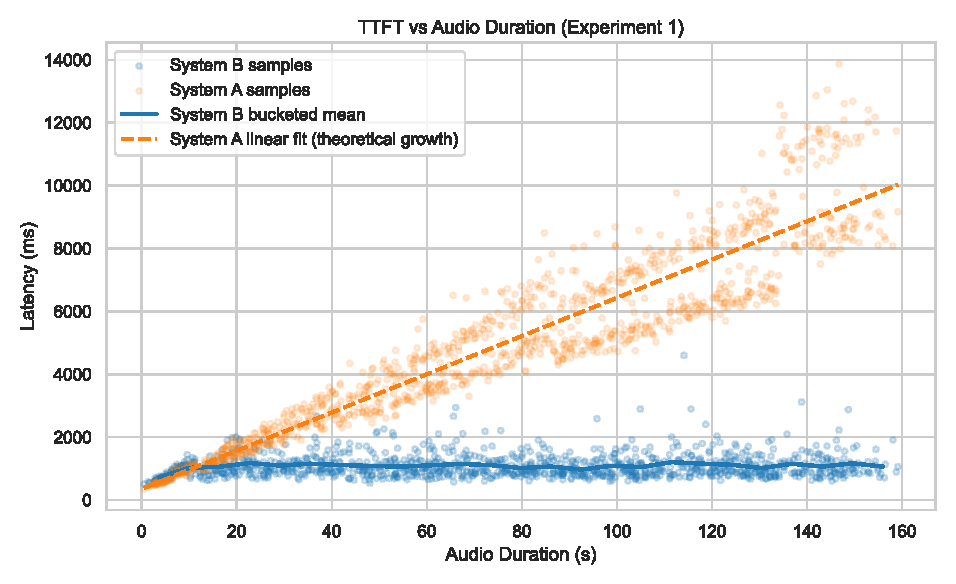
\includegraphics[width=0.55\linewidth]{media/media/image77.pdf}
\caption{TTFT trends of System A and System B over input duration}
\label{fig:trend}
\end{figure}

\subsubsection{Latency Trends}

First-token latency is the core measure of conversational fluency. Figure~\ref{fig:trend} plots the TTFT trajectories of the non-streaming baseline and our streaming system across input durations.

The X-axis is true audio duration (seconds) and the Y-axis end-to-end TTFT (milliseconds). The System~A curve rises near-monotonically with duration, reflecting accumulated post-endpoint serial waiting; System~B flattens from the Long group upward, exhibiting an approximate upper bound dominated by the fixed chunk granularity and tail scheduling overhead. The two curves cross near 15 seconds, where the coverage gains of streaming parallelism begin to outweigh its fixed overhead.

\begin{table}[htbp]
\centering
\caption{TTFT statistics across speech duration groups}
\label{tab:ttft}
\setlength{\tabcolsep}{4pt}
\begin{tabular}{cccccc}
\toprule
Group & Samples & \begin{tabular}{@{}c@{}}Mean\\duration (s)\end{tabular} & \begin{tabular}{@{}c@{}}Streaming\\TTFT (ms)\end{tabular} & \begin{tabular}{@{}c@{}}Non-streaming\\TTFT (ms)\end{tabular} & \begin{tabular}{@{}c@{}}Improvement\\(\%)\end{tabular} \\
\midrule
Short & 35 & 3.44 & 648.17 & 533.42 & -21.5 \\
Medium & 89 & 9.25 & 959.53 & 923.42 & -3.9 \\
Long & 121 & 22.16 & 1126.63 & 1722.04 & 34.6 \\
Very Long & 208 & 45.21 & 1099.16 & 3191.97 & 65.6 \\
Extra Long & 679 & 105.73 & 1087.70 & 6753.43 & 83.9 \\
\bottomrule
\end{tabular}
\end{table}

Table~\ref{tab:ttft} reports TTFT statistics by duration group. The TTFT of the non-streaming baseline System~A grows markedly with input duration: the Short-group mean is 533.42~ms, rising to 1722.04~ms for Long and further to 3191.97~ms and 6753.43~ms for Very Long and Extra Long. This matches the expectation for the cascaded paradigm: ASR must wait for the speech to finish before full decoding, after which the LLM prefills the complete transcript in one shot; the post-endpoint computation chain barely overlaps, making TTFT essentially linear in speech length. The streaming System~B instead shows an approximately constant upper bound from the Long group upward: the Long, Very Long, and Extra Long means are 1126.63~ms, 1099.16~ms, and 1087.70~ms, stable around 1.1~s. The corresponding TTFT reductions over the baseline in these three groups are 34.6\%, 65.6\%, and 83.9\%, with an average absolute reduction of 5.67~s in the Extra Long group---a clear relief of the silent wait in long-speech interaction. By ``constant'' we mean that the dominant term shifts from full computation accumulating with duration to the sum of tail processing and scheduling overhead of the last few chunks; with a 500~ms chunk length and fixed computing resources, TTFT no longer grows appreciably with input duration.

Notably, in the Short and Medium groups System~B shows latency increases of 114.75~ms and 36.11~ms over System~A. We define the latency change as $\Delta \mathrm{TTFT}=\mathrm{TTFT}_{\mathrm{SystemB}}-\mathrm{TTFT}_{\mathrm{SystemA}}$, so $\Delta \mathrm{TTFT}>0$ indicates the streaming design's TTFT exceeds the non-streaming baseline (a negative gain) and $\Delta \mathrm{TTFT}<0$ indicates a latency reduction. For short speech, the fixed overheads of the streaming architecture---chunked processing, cache maintenance, incremental prompt construction---are not offset by parallelization gains, while short audio and text inputs have not yet triggered the long-context prefill bottleneck. The practical implication is adaptive path selection at deployment time: inputs predicted to be short should take the traditional one-shot path, reserving the streaming parallel mechanism for long speech with duration $T\geq 15\,\mathrm{s}$ to obtain the best overall interaction experience.

\subsection{Experiment 2: Ablation}

\subsubsection{Setup}

To quantify the relative contributions of streaming ASR and LLM incremental prefilling, we sampled 50 utterances per group from the Long group upward. Following the grouping defined earlier, we selected the Long (15--30~s), Very Long (30--60~s), and Extra Long ($\geq$60~s) groups, where the benefit of streaming is most visible. Three configurations are compared: Baseline (System~A, both ASR and LLM non-streaming and serial), Streaming ASR Only (ASR streamed; the LLM waits for the full text before starting inference), and Full Streaming (Streaming ASR Only plus LLM incremental prefilling, i.e., System~B).

The core metric is TTFT; logs additionally record the post-endpoint ASR tail-processing time and the LLM prefill time to identify bottlenecks. To make the perceived-latency impact of the architectural differences explicit, we report the mean TTFT of the three configurations and the derived ASR gain and KV-cache gain (positive values shorten TTFT; negative values add cost), so that conclusions are attributable to the targeted mechanisms.

\begin{table}[htbp]
\centering
\caption{Ablation results of core modules}
\label{tab:ablation}
\setlength{\tabcolsep}{4pt}
\begin{tabular}{ccccccc}
\toprule
Group & \begin{tabular}{@{}c@{}}Mean\\duration (s)\end{tabular} & \begin{tabular}{@{}c@{}}Baseline\\TTFT (ms)\end{tabular} & \begin{tabular}{@{}c@{}}Streaming ASR\\Only TTFT (ms)\end{tabular} & \begin{tabular}{@{}c@{}}Full Streaming\\TTFT (ms)\end{tabular} & \begin{tabular}{@{}c@{}}ASR\\gain (ms)\end{tabular} & \begin{tabular}{@{}c@{}}KV Cache\\gain (ms)\end{tabular} \\
\midrule
Long & 21.51 & 1698.88 & 1064.18 & 1084.17 & 634.70 & -19.99 \\
Very Long & 42.43 & 3300.58 & 1171.02 & 1154.06 & 2129.56 & 16.96 \\
Extra Long & 83.75 & 6518.40 & 1228.77 & 1114.57 & 5289.63 & 114.20 \\
\bottomrule
\end{tabular}
\end{table}

\subsubsection{Quantifying Contributions}

Table~\ref{tab:ablation} shows that, under the platform's hardware and models, ASR streaming is the primary source of TTFT reduction. Relative to Baseline, Streaming ASR Only cuts 634.70~ms, 2129.56~ms, and 5289.63~ms in the Long, Very Long, and Extra Long groups---reductions of 37.4\%, 64.5\%, and 81.1\%. In the traditional serial chain, the dominant post-endpoint cost is thus ASR processing of the whole audio; streaming ASR moves most of that computation forward to overlap with the user's speech, sharply compressing post-endpoint work. Incremental prefilling on the LLM side shows a clear length dependence. In the Long group, Full Streaming actually increases TTFT by 19.99~ms over Streaming ASR Only (KV gain $-19.99$~ms): when the context is not yet long enough, the extra costs of incremental calls, cache management, and synchronization can exceed the one-shot prefill computation they save. In the Very Long and Extra Long groups the KV gains are 16.96~ms and 114.20~ms, and in Extra Long the KV cache accounts for about 9.3\% of the overall benefit (114.20/1228.77), indicating that the prefill saving grows with input text and context length.

Combining both mechanisms, Full Streaming holds mean TTFT around 1.1~s (Long 1084.17~ms, Very Long 1154.06~ms, Extra Long 1114.57~ms), reductions of roughly 36.2\%, 65.0\%, and 82.9\% over Baseline. This is consistent with the overall trend: streaming parallelism substantially reduces the waiting time of cascaded systems as input length grows, though the marginal benefit of KV-cache prefilling remains sensitive to engineering details and to hardware concurrency and compute. The ablation also shows that on this platform, running Whisper is already demanding, whereas Qwen2-7B-Instruct is a small model by LLM standards, with far less inference computation than high-end models (often hundreds of billions of parameters or more), so the platform's compute suffices for it. With a mainstream state-of-the-art model, the benefit of incremental KV-cache prefilling should become considerably more pronounced. Another notable observation across the three ascending-length groups: with streaming ASR plus one-shot prefill, processing time still increases with length; with full streaming (KV cache), the three groups show no increasing relationship. This indicates that, in our environment, the quadratic complexity of prefilling the full transcript exceeds the hardware's parallel-computing ceiling and requires increasingly long attention computation, whereas with the KV cache the tail computation is near-linear relative to the full text and stays below the ceiling---so processing time does not grow even as length increases, confirming that incremental KV-cache prefilling meaningfully cuts computation in long-speech scenarios.

\subsection{Experiment 3: Accuracy and Quality Boundary}

\subsubsection{Setup and Evaluation Method}

With latency sharply compressed, the main cost of streaming falls on context truncation and endpoint uncertainty. Unlike System~A, which can exploit the entire audio, streaming ASR sees only a local slice per input fragment, so substitutions, insertions, and omissions become more likely near sentence-final boundaries. To stabilize recognition, the ASR side uses sliding-window context management: a prefix supplies historical audio and a suffix supplies subsequent audio, trading accuracy against tail latency. Using this mechanism, the experiment compares three configurations: prefix=1, suffix=0 (default); prefix=1, suffix=1 (one extra look-ahead segment to improve sentence endings); and prefix=0, suffix=0 (all context removed for minimum latency). We sampled 50 utterances each from the Medium, Long, and Very Long groups (150 in total) to cover the main medium-to-long speech scenarios. We use the standard WER and CER metrics, computed separately for the English (MultiWOZ) and Chinese (CrossWOZ) samples, with the non-streaming full-audio System~A as an upper-bound reference, and compare System~B's recognition quality and tail latency across the streaming context configurations.

\subsubsection{Accuracy--Latency Analysis}

\begin{table}[htbp]
\centering
\caption{Accuracy and processing time under different context-window configurations}
\label{tab:context}
\setlength{\tabcolsep}{4pt}
\begin{tabular}{cccccc}
\toprule
Context configuration & \begin{tabular}{@{}c@{}}MultiWOZ\\WER\end{tabular} & \begin{tabular}{@{}c@{}}MultiWOZ\\CER\end{tabular} & \begin{tabular}{@{}c@{}}CrossWOZ\\WER\end{tabular} & \begin{tabular}{@{}c@{}}CrossWOZ\\CER\end{tabular} & \begin{tabular}{@{}c@{}}ASR time\\(ms)\end{tabular} \\
\midrule
prefix 1 + suffix 1 & 0.0895 & 0.0196 & 0.0083 & 0.0203 & 1327.48 \\
prefix 1 + no suffix (default) & 0.0813 & 0.0221 & 0.0118 & 0.0292 & 1224.96 \\
prefix 0 + suffix 0 & 0.0619 & 0.0226 & 0.0210 & 0.0500 & 1086.16 \\
\bottomrule
\end{tabular}
\end{table}

Each context configuration covers 150 samples: 74 from MultiWOZ and 76 from CrossWOZ. Because the evaluation audio is TTS-synthesized from the original dialogue text, we use the pre-synthesis text as the reference transcript and normalize both ASR output and reference before computing WER/CER---unifying case, punctuation, whitespace, and Chinese/English tokenization---then align by edit distance. On this synthetic speech collection, the non-streaming System~A transcribing complete audio yields WER/CER near zero, indicating high consistency between reference text and synthesized audio under this setup; this serves only as an upper-bound reference for this batch of synthetic data and does not imply the model is error-free on open real-world speech. To further reduce bias from synthesis and alignment, samples with anomalous metrics were re-checked, and the analysis focuses on relative differences across context configurations.

Table~\ref{tab:context} compares accuracy and tail latency across the context-window configurations. Adding both prefix and suffix (pre1\&suf1) improves Chinese sentence-final stability most visibly: CrossWOZ WER/CER drop from the default 0.0118/0.0292 to 0.0083/0.0203. The longer processed fragments raise the post-endpoint tail time, increasing \texttt{asr\_time\_ms} from 1224.96~ms to 1327.48~ms (+102.52~ms), consistent with the mechanism that a suffix window must wait for extra audio and perform more decoding. For English MultiWOZ, adding the suffix lowers CER from 0.0221 to 0.0196 but slightly raises WER to 0.0895, suggesting that under word-level scoring the suffix window's effects on alignment and tokenization become more sensitive; this warrants further verification with real recordings and larger samples. Removing all extra context (pre0\&suf0) achieves the lowest time (\texttt{asr\_time\_ms} down to 1086.16~ms, 138.80~ms below default), while Chinese errors grow markedly as expected: CrossWOZ CER rises to 0.0500 and WER to 0.0210. The historical context provided by the prefix thus exerts an important constraint in streaming recognition, giving the audio--language model stronger local corrective power and suppressing the error accumulation of long sentences.

Because Chinese is character-based while English is word-based, we focus on CER for the Chinese dataset and WER for the English one. On Chinese, CER clearly decreases as context grows; on English, WER is essentially flat across the three configurations, and the minimum-context configuration's lowest WER can be treated as experimental fluctuation. The reason is that Chinese has many homophones, so added context materially helps transcribe the correct characters, whereas English homophones are far fewer---given accurate pronunciation, word-level recognition is comparatively stable and extra context brings no significant accuracy gain. In deployment, English dialogue can therefore drop the prefix/suffix extensions and push the streaming architecture's latency advantage to the limit.

Finally, from the end-to-end latency budget: Experiments 1 and 2 show that TTFT for Long-and-above speech can be held near 1.1~s, and the 0.1--0.2~s tail costs of the context configurations in Table~\ref{tab:context} already occupy a nontrivial share. The choice is scenario-dependent: Chinese tasks that are more accuracy-sensitive can enable pre1\&suf1 to reduce sentence-final errors, while pre0\&suf0 serves as an ultra-low-latency mode or for English dialogue. Given that conversational LLMs are generally robust to semantic-level noise, small transcript errors are unlikely to noticeably affect LLM reasoning. Future work can introduce semantic-consistency and task-completion metrics to quantify directly the semantic drift caused by transcription errors.

\section{Conclusion and Outlook}

\subsection{Summary}

Addressing the excessive post-endpoint waiting of cascaded voice dialogue systems on long speech input, this paper designs and implements a low-latency voice dialogue architecture based on pipeline parallelism. With streaming computation and state incrementalization as the design principles, it converts the full ASR transcription and one-shot LLM prefilling of the traditional serial chain into overlappable streaming processes: on the ASR side, VAD segmentation, a sliding window, and prefix/suffix context wrap the offline-oriented Whisper into a streaming module that emits stable incremental text; on the LLM side, \texttt{past\_key\_values} enables incremental prefilling of new text fragments, and the last-step \texttt{logits} of the prefill phase are reused to launch first-token decoding. This strategy does not change the complexity order of attention computation; rather, it moves prefill computation that would otherwise concentrate after the end-of-speech endpoint into the user's speaking time, cutting the post-endpoint critical path.

Experiments confirm the architecture's effectiveness. On the long-speech dataset built from MultiWOZ and CrossWOZ, our system holds a stable advantage over the traditional non-streaming baseline in duration groups above 15 seconds, keeping TTFT within a stable range, while sliding-window context preserves transcription accuracy with WER/CER in an acceptable range. Although TTFT in the Long-and-above groups remains around 1.1~s---still short of the roughly 200~ms turn-taking gap of human conversation~\cite{ref21}---its greatest advantage over the serial design is that long-speech TTFT stops growing with utterance length once it reaches its plateau. With more efficient inference hardware, lower-latency ASR models, and further scheduling optimization to compress the remaining post-endpoint wait, response latency matching the human conversational gap should become attainable for speech of any length.

\subsection{Limitations}

Despite the reduction in post-endpoint waiting on long speech, the system remains bound by the cascaded architecture. First, the prototype still follows the half-duplex turn-taking pattern of user speaks--system processes--system replies, and cannot yet handle the overlapping speech and interruptions of natural conversation~\cite{ref22}. Second, text remains the sole interface between ASR and the LLM, so paralinguistic information---intonation, emotion, pauses---is lost in transcription. Third, the test audio is mainly TTS-synthesized; robustness under real noise, accents, and microphone conditions requires further validation.

\subsection{Future Work}

Future work will focus on two directions. First, suppressing tail-latency jitter: experiment logs show that peak latency for some long-speech samples comes from consecutive segment triggers at the end of the utterance; tail merging, queue back-pressure, and adaptive scheduling could reduce redundant ASR inference. Second, improving end-of-turn detection: real dialogue typically relies on silence thresholds to decide whether the user has finished speaking, and once model-side TTFT is compressed to about 1~s, the fixed silence wait becomes the new dominant term. A lightweight semantic end-of-utterance (EOU) model, combining streaming ASR text with context to predict whether the turn is semantically complete, could further reduce real-world interaction waiting.

\begin{thebibliography}{22}
\bibitem{ref1} OpenAI. GPT-4o system card[EB/OL]. 2024. https://arxiv.org/abs/2410.21276.
\bibitem{ref2} TAN Z H, SARKAR A K, DEHAK N. rVAD: an unsupervised segment-based robust voice activity detection method[J]. Computer Speech \& Language, 2020, 59: 1-21.
\bibitem{ref3} PRABHAVALKAR R, HORI T, SAINATH T N, et al. End-to-end speech recognition: a survey[J]. IEEE/ACM Transactions on Audio, Speech, and Language Processing, 2024, 32: 325-351.
\bibitem{ref4} VASWANI A, SHAZEER N, PARMAR N, et al. Attention is all you need[C]//Advances in Neural Information Processing Systems. Red Hook: Curran Associates, 2017, 30: 5998-6008.
\bibitem{ref5} LI J. Recent advances in end-to-end automatic speech recognition[J]. APSIPA Transactions on Signal and Information Processing, 2022, 11(1). DOI: 10.1561/116.00000050.
\bibitem{ref6} RADFORD A, KIM J W, XU T, et al. Robust speech recognition via large-scale weak supervision[C]//Proceedings of the 40th International Conference on Machine Learning. PMLR, 2023, 202: 28492-28518.
\bibitem{ref7} ZHENG Y, CHEN Y, QIAN B, et al. A review on edge large language models: design, execution, and applications[J]. ACM Computing Surveys, 2025, 57(8): 209.
\bibitem{ref8} ZHU X, LI J, LIU Y, et al. A survey on model compression for large language models[J]. Transactions of the Association for Computational Linguistics, 2024, 12: 1556-1577.
\bibitem{ref9} TAY Y, DEHGHANI M, BAHRI D, et al. Efficient transformers: a survey[J]. ACM Computing Surveys, 2022, 55(6): 109.
\bibitem{ref10} SETHIYA N, MAURYA C K. End-to-end speech-to-text translation: a survey[J]. Computer Speech \& Language, 2025, 90: 101751.
\bibitem{ref11} YIN S, FU C, ZHAO S, et al. A survey on multimodal large language models[J]. National Science Review, 2024, 11(12): nwae403.
\bibitem{ref12} MOHAMED A, LEE H Y, BORGHOLT L, et al. Self-supervised speech representation learning: a review[J]. IEEE Journal of Selected Topics in Signal Processing, 2022, 16(6): 1179-1210.
\bibitem{ref13} Silero Team. Silero VAD: pre-trained enterprise-grade voice activity detector[EB/OL]. 2024. https://github.com/snakers4/silero-vad.
\bibitem{ref14} BUDZIANOWSKI P, WEN T H, TSENG B H, et al. MultiWOZ: a large-scale multi-domain Wizard-of-Oz dataset for task-oriented dialogue modelling[C]//Proceedings of EMNLP 2018. Stroudsburg: Association for Computational Linguistics, 2018: 5016-5026.
\bibitem{ref15} ZHU Q, HUANG K, ZHANG Z, et al. CrossWOZ: a large-scale Chinese cross-domain task-oriented dialogue dataset[J]. Transactions of the Association for Computational Linguistics, 2020, 8: 281-295.
\bibitem{ref16} TAN X, CHEN J, LIU H, et al. NaturalSpeech: end-to-end text-to-speech synthesis with human-level quality[J]. IEEE Transactions on Pattern Analysis and Machine Intelligence, 2024, 46(6): 4234-4245.
\bibitem{ref17} DU Z, CHEN Q, ZHANG S, et al. CosyVoice: a scalable multilingual zero-shot text-to-speech synthesizer based on supervised semantic tokens[EB/OL]. 2024. https://arxiv.org/abs/2407.05407.
\bibitem{ref18} NI J, YOUNG T, PANDELEA V, et al. Recent advances in deep learning based dialogue systems: a systematic survey[J]. Artificial Intelligence Review, 2023, 56(4): 3055-3155.
\bibitem{ref19} ZHANG Z, TAKANOBU R, ZHU Q, et al. Recent advances and challenges in task-oriented dialog systems[J]. Science China Technological Sciences, 2020, 63(10): 2011-2027.
\bibitem{ref20} YANG A, YANG B, HUI B, et al. Qwen2 technical report[EB/OL]. 2024. https://arxiv.org/abs/2407.10671.
\bibitem{ref21} STIVERS T, ENFIELD N J, BROWN P, et al. Universals and cultural variation in turn-taking in conversation[J]. Proceedings of the National Academy of Sciences, 2009, 106(26): 10587-10592.
\bibitem{ref22} SKANTZE G. Turn-taking in conversational systems and human-robot interaction: a review[J]. Computer Speech \& Language, 2021, 67: 101178.
\end{thebibliography}

\end{document}
